\documentclass[12pt]{article}
\usepackage[czech]{babel}
\usepackage[utf8]{inputenc}
\usepackage[IL2]{fontenc}
\usepackage{wrapfig}
\usepackage{graphicx}
\usepackage{listings}
\usepackage{amsmath}
\usepackage{scrextend}
\usepackage{cprotect}
\usepackage{float}
\usepackage{hyperref}
\usepackage{indentfirst}
\newcommand{\htmltag}[1]{%
	\scalebox{.6}[1]{$<$}{\ttfamily#1}\scalebox{.6}[1]{$>$}%
}

\begin{document}
\pagenumbering{gobble} %bez cisel
\begin{titlepage}
\centerline{
\includegraphics[width=10cm]{img/logo.jpg}}
\begin{center}
\vspace{30px}
{\Huge
\textbf{Semestrální práce KIV/UIR}\\
\vspace{1cm}
}
{\Large
\textbf{Klasifikace dokumentů}\\
}
\vspace{1cm}
{\large
Pavel Třeštík\\
}
{\normalsize
A17B0380P
}
\end{center}
\vspace{\fill}
\hfill
\begin{minipage}[t]{7cm}
\flushright
\today
\end{minipage}
\end{titlepage}

\tableofcontents
\newpage
\pagenumbering{arabic} %
%
% Zadání
%
\section{Zadání}
Ve zvoleném programovacím jazyce navrhněte a implementujte program, který umožní klasifikovat textové dokumenty do tříd podle jejich obsahu, např. počasí,     sport, politika, apod. Při řešení budou splněny následující \\
podmínky:
\begin{itemize}

\item Použijte data z českého historického periodika Posel od Čerchova“, která jsou k dispozici na \url{https://drive.google.com/drive/folders/1mQbBNS43gW    FRMHDYdSkQug47cuhPTsHJ?usp=sharing}. V původní podobě jsou data k dispozici na \url{http://www.portafontium.eu/periodi\\cal/posel-od-cerchova-1872?languag    e=cs.}

\item Pro vyhodnocení přesnosti implementovaných algoritmů bude NUTNÉ vybrané dokumenty ručně označkovat. Každý student ručně anotuje 10 stran zadaného te    xtu –
termín 31.3.2020. Za dodržení termínu obdrží student bonus 10b.

\item Přiřazení konkrétních textů jednotlivým studentům spolu s návodem na anotaci a příklady je uloženo spolu s daty na výše uvedené adrese, konkrétně:
        \begin{itemize}
        \item 0 - vzorová složka (takhle by měl výsledek vypadat)
        \item 1, 2, .. , 15, 101, 102, .. - data k anotaci
        \item přiřazení souboru studentum.xlsx - určení, jaké soubory má jaký student   anotovat. Až budete mít anotaci hotovou, doplňte sem informaci.
        \item Anotační příručka - návod, jak články anotovat.
        \item Klasifikace dokumentů - kategorie.xlsx - seznam kategorií k anotaci s příklady.
        \item sem prace20.pdf - Zadání semestrální práce
        \end{itemize}

\item implementujte alespoň tři různé algoritmy (z přednášek i vlastní) pro tvorbu příznaků reprezentující textový dokument.

\item implementujte alespoň dva různé klasifikační algoritmy (klasifikace\\ s učitelem):
        \begin{itemize}
        \item Naivní Bayesův klasifikátor
        \item klasifikátor dle vlastní volby
        \end{itemize}

\item funkčnost programu bude následující:
– spuštění s parametry:\\
\textbf{název klasifikátoru, soubor se seznamem klasifikačních tříd, trénovací množina, testovací množina, parametrizační algoritmus, klasifikační algorit    mus,název modelu}\\
program natrénuje klasifikátor na dané trénovací množině, použije zadaný parametrizační a klasifikační algoritmus, zároveň vyhodnotí úspě- šnost klasifika    ce a natrénovaný model uloží do souboru pro pozdější použití (např. s GUI).– spuštění s jedním parametrem:\\
\textbf{název klasifikátoru, název modelu} \\
program se spustí s jednoduchým GUI a uloženým klasifikačním modelem. Program umožní klasifikovat dokumenty napsané v GUI pomocí klávesnice (resp. překopí    rované ze schránky).

\item ohodnoťte kvalitu klasifikátoru na dodaných datech, použijte metriku přesnost (accuracy), kde jako správnou klasifikaci uvažujte takovou, kde se kla    sifikovaná třída nachází mezi anotovanými. Otestujte všechny konfigurace klasifikátorů (tedy celkem 6 výsledků).
\end{itemize}


Poznámky:
\begin{itemize}
\item pro vlastní implementaci není potřeba čekat na dokončení anotace. Pro průběžné testování můžete použít korpus současné češtiny, který je k dispozici     na \url{http://ctdc.kiv.zcu.cz/} (uvažujte pouze první třídu dokumentu podle názvu, tedy např.
dokument 05857 zdr ptr eur.txt náleží do třídy zdr“ - zdravotnictví).
”
\item další informace, např. dokumentace nebo forma odevzdávání jsou\,k dispozici na CW pod záložkou Samostatná práce.

\end{itemize}
%
% Analýza problému
%
\pagebreak
%
\section{Analýza úlohy}
\subsection{Algoritmy pro tvorbu příznaků}
Existuje řada metod získávání informací (modelů) z rozdílných typů dat.
Pro tuto
práci nás ale zajímají pouze jazykové pravděpodobnostní modely. Ty se
řadí do několika tříd: unigram, n-gram, exponenciální, neuronové sítě
a ostatní (takové, které nepřipadají do ani jedné z předchozích skupin).\\
Ve skutečnosti ale některé třídy jsou založeny na jiné třídě. Na
příklad unigram je ve skutečnosti n-gram pro jednotlivá slova. Mezi
nejvýznačnější reprezentanty patří \texttt{Bag of Words},
\texttt{Bigram}, \texttt{Trigram} a \texttt{Word2vec}.
\subsubsection{Bag of Words}
Prvním z algoritmů, které jsem vybral je \texttt{Bag of Words}. Jedná
se o unigram, tudíž každý text/ dokument je reprezentován jednotlivými
slovy. Slova jsou ukládána do slovníku a jednotlivé klasifikační třídy/
dokumenty
jsou reprezentovány vektory o délce slovníku. Hodnoty vektorů jsou
reprezentací četností výskytu slov v textu/ dokumentu pro každou
klasifikační třídu (nebo jednotlivé dokumenty). Toto ovšem 
vytváří problém, kdy při objemné množině slov ve slovníku, se jich pouze
malá část vyskytuje ve vektoru reprezentující klasifikační třídu/
dokument.

Příklad \texttt{Bag of Words}\\
Zdroj (Wikipedia): \url{https://en.wikipedia.org/wiki/Bag-of-words\_model} \\
%\hrulefill\\
\rule{\textwidth}{0.4pt}
	\textbf{Texty}\\
	\texttt{(1) John likes to watch movies. Mary likes movies too.}\\
	\texttt{(2) Mary also likes to watch football games.}\\

	\textbf{Rozdělení textů}\\
	\texttt{BoW1 = \{"John":1,"likes":2,"to":1,"watch":1,"movies":2,"Mary":1,\\"too":1\};}\\
	\texttt{BoW2 = \{"Mary":1,"also":1,"likes":1,"to":1,"watch":1,"football":1,\\"games":1\};}\\

	\textbf{Slovník textů}\\
	\texttt{BoW3 = \{"John":1,"likes":3,"to":2,"watch":2,\\"movies":2,"Mary":2,"too":1,"also":1,"football":1,"games":1\};}\\

	%\pagebreak
	\textbf{Vektory reprezentující texty}\\
	\texttt{(1) [1, 2, 1, 1, 2, 1, 1, 0, 0, 0]}\\
	\texttt{(2) [0, 1, 1, 1, 0, 1, 0, 1, 1, 1]}\\
\rule{\textwidth}{0.4pt}
\subsubsection{Bigram}
Druhým algoritmem pro tvorbu příznaků bude \texttt{Bigram}. Ačkoliv 
\texttt{Bag of Words} je ve skutečnosti n-gram pro n = 1 a \texttt{Bigram}
je n-gram pro n = 2 je v těchto algoritmech značný rozdíl. \texttt{Bigram}
páruje slova a počítá pravděpodobnost páru jako podmíněnou pravděpodobnost
obou slov páru.

Pravděpodobnost výrazu je spočítána podle vztahu na Obrázku
\ref{fig:bigram_prob}.
Párování slov je ukázáno na následujícím příkladu.\\
\rule{\textwidth}{0.4pt}
	\textbf{Věta}\\
	\texttt{Tato věta je příklad.}\\

	\noindent\textbf{Bigramy}\\
	\texttt{bigrams = \{"S, Tato", "Tato, věta", "věta, je", "je, příklad",\\ "příklad, /S\}}\\

	\noindent S = začátek věty,
	/S = konec věty\\
\rule{\textwidth}{0.4pt}
\begin{figure}[H]
        \centering
        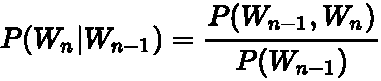
\includegraphics[]{img/bigram_prob.pdf}
        \caption{Pravděpodobnost výrazu bigramu}
        Zdroj: \url{https://en.wikipedia.org/wiki/Bigram}
        \label{fig:bigram_prob}
\end{figure}
\subsubsection{TF-IDF}
Posledním vybraným algoritmem je TF-IDF. Na rozdíl od předchozích dvou
vybraných algoritmů nevytváří příznaky z textu, ale upravuje již 
existující příznaky, tudíž je využíván spolu s \texttt{Bag of Words}.
Algoritmus ohodnotí jednotlivá slova váhou místo jejich četností.
Čím častěji se slovo v textech/ dokumentech vyskytuje, tím nižší váhu
má po TF-IDF. Tento algoritmus svým způsobem "vytváří" takzvané 
\textbf{stop words}. To jsou slova, které v jazyce pro klasifikaci
nemají žádný význam (na příklad pro Český jazyk slova jako: a, pro, 
nebo...).
%
\subsection{Klasifikační algoritmy}
Výběr klasifikačního algoritmu značně závisí na účelu našeho 
projektu. Z mnoha klasifikátorů jako je \texttt{Naive Bayes},
\texttt{Support Vector Machine (SVM)}, \texttt{Linear regression},
\texttt{Neural Networks} a dalších, potřebujeme vybrat podle potřeb.
Nejdůležitějšími vlastnostmi klasifikátoru při výběru jsou jeho 
přesnost (accuracy), složitost a rychlost.
\subsubsection{Naive Bayes}
Je jeden z nejrychlejších a
a nejjednodušších klasifikátorů. Jeho nedostatkem je, že potřebuje
poměrně přesná trénovací data, aby jeho klasifikace byly co 
možná nejpřesnější.

Klasifikátor vybere nejpravděpodobnější třídu podle následujícího
vztahu (viz Obrázek \ref{fig:nb_class}).
\begin{figure}[H]
        \centering
        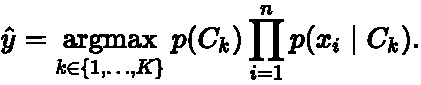
\includegraphics[]{img/nb_class.pdf}
        \caption{Rovnice vybrání třídy}
        Zdroj: \url{https://en.wikipedia.org/wiki/Naive\_Bayes\_classifier}
        \label{fig:nb_class}
\end{figure}
\subsubsection{k-nearest neighbors}
Převede klasifikovaný text/ dokument na vektor a spočítá vzdálenost
ke\,každému 
trénovacímu textu/ dokumentu. Poté přiřadí klasifikovanému
textu třídu, která má nejvíce zástupců v určité blízkosti. Tento
algoritmus je velmi jednoduchý a poměrně rychlý. Nevýhodou je přesnost,
která pokud trénovací soubory nemají jednoznačně určenou třídu, není
velmi vysoká.

Příklad klasifikace: zelená tečka na Obrázku \ref{fig:knn}. Zelená 
tečka bude klasifikována jako červený trojúhelník, protože v okolí
jsou 2 červené trojúhelníky a pouze 1 modrý čtverec.
\begin{figure}[H]
        \centering
        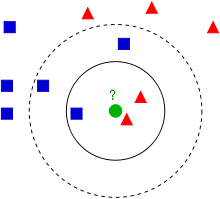
\includegraphics[]{img/knn.png}
        \caption{Příklad klasifikace k-nn}
        Zdroj: \url{https://en.wikipedia.org/wiki/K-nearest\_neighbors\_algorithm}
        \label{fig:knn}
\end{figure}
%
% Implementace
%
\section{Implementace}
Pro tento projekt jsem zvolil jazyk Python. Důvodem bylo,
že pro umělou inteligenci je pro Python množství knihoven.
Naneštěstí jsem se k využití žádné z knihoven nedostal.
\subsection{Bag of Words}
Původně jsem tento model implementoval 
použitím teoretického způsobu. Neboli vytvořil jsem 
slovník a podle toho reprezentoval třídy jako vektory.
Toto ale trvalo přibližně 15 vteřin.

Nakonec jsem začal jednotlivé třídy reprezentovat pomocí
Python struktury \textbf{dictionary}. Tato struktura proces
proces vytváření vektorů tříd urychlila na méně než vteřinu,
ale není třeba dodržovat původní model a slovník není vůbec
potřeba. Výhoda absence slovníku je, že každá třída nemá
značné množství nul za slova, která se ve třídě nevyskytují.
\subsection{Bigram}
Také reprezentován pomocí struktury \textbf{dictionary}.
Vytvářen velmi podobně jako \texttt{Bag of Words}, ale 
klíče slovníku jsou 2 slova oddělená mezerou.

Má změna o proti teoretickému způsobu algoritmu je v
počítání pravděpodobnosti. Stejně jako u \texttt{Bag of Words},
jsou počítány pouze četnosti jednotlivých bigramů v textu.
Pravděpodobnost je potom v klasifikátoru počítána jako 
\texttt{počet četností/ počet bigramů ve třídě}, což není
správný způsob počítání pravděpodobnosti bigramu.
\subsection{TF-IDF}
Provádí výpočty přesně jak má. Implementován tak, aby
počítal nad strukturou \textbf{dictionary}.

Navíc jsem se pokusil algoritmus doplnit o "normalizaci",
se kterou lehce zvýší přesnost na poskytnutých datech.

Je možné použít originální i mou "normalizovanou"
metodu, ale musí se přepnout ve zdrojovém kódu.
\subsection{Naive Bayes}
Implementován pro práci nad strukturou \textbf{dictionary}. Z důvodu
velkého počtu slov ve třídách, čímž vznikaly pravděpodobnosti
s příliš mnoho desetinnými místy pracuje v logaritmovaném prostoru.
Místo násobení pravděpodobností, sčítá logaritmy pravděpodobností.
Také používá tak zvaný \textbf{Laplace smoothing}, díky čemuž
i slova, která se ve třídě nevyskytují mají malý vliv na 
klasifikaci místo nulového.
\subsection{k-nearest neighbors}
Pro tento algoritmus bylo třeba upravit příznakové metody, 
aby místo s jedním slovníkem definujícím třídu, vytvářely
list souborů definující danou třídu.

Díky této úpravě může algoritmus fungovat přesně jak je 
popsán v analýze úlohy.
%
% Uživatelská dokumentace
%
\section{Uživatelská dokumentace}
Program se spouští z konzole. Program je spustitelný na verzi Python
2.x. Program má Console mód a GUI mód. Console mód natrénuje 
klasifikátor a klasifikuje testovací množinu. GUI mód otevře
jednoduché GUI okno kam uživatel vloží text, který chce klasifikovat.
Aby se rozlišilo jestli se program spouští v příkazové řádce
nebo v GUI má 2 rozdílné zpracování argumentů. Proto je nutno 
specifikovat, který použít, formou argumentu.
\subsection{Konzolový mód}
Program se spustí následujícím způsobem: 
\textbf{python main.py Console [-h] classes\_name\_file train\_files test\_files irs classifier model\_name}
\begin{itemize}
	\item \textbf{Console} -- argument specifikující, které zpracování argumentů
		použít.
	\item \textbf{[-h]} -- dobrovolný argument, při jehož použití se vypíše
		nápověda k ostatním argumentům.
	\item \textbf{classes\_name\_file} -- soubor s listem klasifikovaných tříd.
		Jeden popisek třídy na každé řádce.
	\item \textbf{train\_files} -- adresář obsahující soubory, ze kterých se 
		vytvoří model klasifikátoru.
	\item \textbf{test\_files} -- adresář obsahující soubory na kterých
		se otestuje model klasifikátoru.
	\item \textbf{irs} -- způsob vytváření příznaků:
		\begin{itemize}
			\item \textbf{bow} -- použije \texttt{Bag of Words}
			\item \textbf{bi} -- použije \texttt{Bigram}
			\item \textbf{bowtfidf} -- použije \texttt{Bag of Words
				+ TF-IDF}
		\end{itemize}
	\item \textbf{classifier} -- který klasifikátor se použije s modelem:
		\begin{itemize}
			\item \textbf{nb} -- použije \texttt{Naive Bayes}
			\item \textbf{knn} -- použije \texttt{k-nearest neighbors}
		\end{itemize}
	\item \textbf{model\_name} -- název souboru, do kterého se model uloží.
\end{itemize}
\subsection{GUI mód}
Spuštění: \textbf{python main.py GUI [-h] model\_name}
\begin{itemize}
	\item \textbf{GUI} -- argument specifikující, které zpracování argumentů
		použít.
	\item \textbf{[-h]} -- dobrovolný argument, při jehož použití se vypíše
		nápověda k ostatním argumentům.
	\item \textbf{model\_name} -- název souboru, ze kterého se načte model,
		který se použije pro klasifikaci textu v grafickém rozhraní.
\end{itemize}
%
% Výsledky
%
\section{Shrnutí výsledků}
Všechny kombinace jsou zahrnuty v následující tabulce (viz Tabulka
\ref{tab:results}).

\begin{table}[H]
	\centering
        \begin{tabular}{| c | c | c |}
                \hline
                Příznaková metoda & Klasifikátor & Přesnost\\
                \hline
		BoW & Naive Bayes & 23.81\% \\
                \hline
                Bigram & Naive Bayes & 15.24\% \\
                \hline
                Bow + TF-IDF & Naive Bayes & 24.76\% \\
                \hline
                BoW & k-nn & 11.43\% \\
                \hline
                Bigram & k-nn & 12.38\% \\
                \hline
                Bow + TF-IDF & k-nn & 9.52\% \\
                \hline
        \end{tabular}
\caption{Tabulka výsledků}
\label{tab:results}
\end{table}
První věcí, která je z výsledků zřejmá, je že žádná přesnost
nedosahuje ani 30\%. Původně jsem očekával výsledky mezi 30\% 
až 60\%. Bohužel těchto výsledků se nepodařilo dosáhnout.
Hlavním důvodem proč jsou výsledky takto nepříznivě je pravděpodobně
velká variace slov a fakt, že v programu nejsou použity žádné 
\textbf{stop words}.

Přesnost by se měla dát zvýšit přidáním \textbf{stop words}.
Dalším způsobem zvýšení přesnosti by bylo ošetřit variaci slov.
Slova z testovacích i trénovacích dat mají díky tomu, že jsou 
skenována OCR, velké množství chyb. To by se\,dalo částečně vylepšit
používáním pouze kořenů slov (tak zvaný \textbf{stemming}). Druhým
způsobem by bylo použít \textbf{word2vec}, který ze slov udělá 
vektory a\,dovolil by shlukovat vektory, které jsou si podobné.
%
% Závěr
%
\section{Závěr}
Program bohužel nedává moc dobré výsledky a nepodařilo se úplně
naplnit mé představy. Myslím si, že by program mohl dosáhnout lepších
výsledků, při použití některé z metod popsaných v předchozí sekci.

Dále by se program dal vylepšit úpravou implementací některých
algoritmů.
%
\end{document}
